\documentclass[a4paper,twoside,12pt, openany]{book}

\usepackage[english]{babel}

\usepackage{fontspec}
\setmainfont{Times New Roman} % Choisissez une fonte sérif lisible (Latin Modern, Junicode, Times)
\usepackage{titlesec}
%Module d'usage facultatif permettant d'intégrer les tables, index, graphie, automatiquement à la table des matières
\usepackage{tocbibind}
%\usepackage{lscape}
\usepackage{amssymb}
\usepackage{amsmath}
\usepackage{graphicx}
\graphicspath{ {./img/} }

\usepackage[margin=2.5cm]{geometry}
\usepackage{setspace}
\setlength{\parindent}{0cm}
\onehalfspacing

%%%Pour les tableaux
%\usepackage{multirow}


%%% Les index
%\usepackage{makeidx}
%\usepackage{multind} %Ou splitidx
%\usepackage{index} %…
%\makeindex
%\makeindex{edition}
%\makeindex{texte}
%\newindex{etude}{adx}{and}{Index de l'étude}
%\newindex{edition}{bdx}{bnd}{Index de l'édition}



%%%Édition critique
%\usepackage{eledmac}
%\usepackage{eledpar}

%\footparagraph{A}

%\renewcommand{\Rlineflag}{D}

\hyphenation{}

\usepackage[babel]{csquotes}

\usepackage[backend=biber, sorting=nyt, style=enc]{biblatex}
\addbibresource{biblio/references.bib}

\defbibheading{secondary-source}{\subsection*{Secondary sources}}
\defbibheading{primary-source}{\subsection*{Primary sources}}

\usepackage{enumerate, lettrine}
\usepackage{enumitem}
\usepackage{hyperref}

\titleformat{\chapter}[display]
{\normalfont\bfseries}{}{-3em}{\Huge \thechapter. }


\title{M1}
\author{Francesco Paolo Savatteri}


\begin{document}


%\begin{abstract}

\frontmatter

\begin{titlepage}
\begin{center}

\bigskip

\begin{large}
UNIVERSITÉ PARIS, SCIENCES \& LETTRES
\end{large}
%TODO: nom établissement de préparation
\begin{center}\rule{2cm}{0.02cm}\end{center}

\bigskip
\bigskip
\bigskip
\begin{Large}
\textbf{Francesco Paolo Savatteri}\\
\end{Large}
\begin{normalsize}
\textit{Diplômé de master}\\
\end{normalsize}

\bigskip
\bigskip
\bigskip

\begin{Huge}
\textbf{M1}\\
\end{Huge}
\bigskip
\bigskip
\begin{LARGE}
\textbf{Evaluating the relationship between far-right and Incel communities on Telegram: a network analysis approach}\\
\end{LARGE}

\bigskip
\bigskip
\bigskip
\begin{large}
\end{large}
\vfill

\begin{large}
Mémoire de première année de master\\
« Humanités numériques et computationnelles » \\
\bigskip
2024
\end{large}

\end{center}
\end{titlepage}

\section*{Abstract}
\addcontentsline{toc}{chapter}{Abstract}

Incels are a loose community of people who are very active on social media and disseminate strongly misogynistic content. Their relationship with the extreme right has often been debated in research articles and in the media. The aim of this research is to investigate the relationship between these two online communities through the analysis of channel networks on Telegram. While most research on the topic clearly focuses on English-speaking communities, this work examines Italian-speaking incels and far-right spheres. \\

The channel networks were created from messages forwarded from one telegram channel to another by snowball sampling from three different sets of seed channels - two far-right channels, two incel channels, two far-left channels (the last to be used as a control example). Two indices were developed to measure the extent to which forwarded message flows are similar for the three networks. The assumption behind this work is that forwarded messages are an indicator of homophily. Thus that if there is a large number of messages forwarded from channel A to channel B and/or vice versa, it is likely that the members of the two channels share the same underlying beliefs and worldviews.\\

The results obtained confirm the existence of a closer link between the incels and far-right spheres than between incels and the far-left. Several aspects remain to be further investigated to validate the results.


\medskip

\textbf{Keywords:} Incel; far-right; alt-right; Telegram; network analysis; online communities; snowball sampling

\textbf{Bibliographic Information:} Francesco Paolo Savatteri, \textit{Evaluating the relationship between far-right and Incel communities on Telegram: a network analysis approach}, M.A. thesis M1 « Digital and computational humanities », dir. Samuel Bouron and Florian Cafiero , Université Paris, Sciences \& Lettres, 2024.


\clearpage
\thispagestyle{empty}
\cleardoublepage

\section*{Bibliography}
\printbibliography[heading=primary-source, keyword=primary-source]
\printbibliography[heading=secondary-source, keyword=secondary-source]
\addcontentsline{toc}{chapter}{Bibliography}


\mainmatter


\chapter{Introduction}

\section{Take the redpill}
A website with a white background and black lettering. No pictures or videos, just a few words linking to other pages. The woman who created it in 1997 is a Canadian student who is known only by her name, Alana. The first entry at the top of the page reads « Alana's Involuntary Celibacy Project ».This is the first time the term \enquote{incel}, a contraction of “Involuntary Celibates,” appears on the Web.\\
It was initially a blog where people of all genders and sexual orientations who were unable to have sexual and romantic relationships could talk about their experiences and support each other. After a few years, however, things changed.\\

Today, the term \enquote{incel} denotes a universe of communities of people active primarily online  – especially male, white, heterosexual people – who are unable to have relationships with women. Although heterogeneous and geographically widespread in many places around the world, the elements shared by the various groups are a very strong misogyny and a distinct worldview.
\\
As Stéphane Baele and his colleagues suggest in a 2021 study, in the incel conception society is divided into classes based on physical appearance. At the top are the minority of highly attractive “Alpha” males (or “Chads”) and females (or “Stacys”). Below them is the majority of average-looking “Betas” (or “normies”), and at the bottom are the minority of unattractive “Incels”, who are exclusively males suffering from “involuntary celibacy”\footcite{baele2021}.\\
Incel communities are part of a larger Internet subculture called the “manosphere”. This can be defined as a collection of misogynist and anti-feminist groups sharing the idea that men are the real victims of a world that is unfairly in favour of
women\footcite{sugiura2021}. In the rhetoric of these communities, accepting this worldview is described as “taking the red pill”, in reference to an iconic scene from the movie The Matrix\footcite{vanvalkenburgh2021}. In this scene, the protagonist Neo is offered a red pill, which opens to knowledge of the truth, or a blue pill, which guarantees blissful ignorance.

\section{Why another research?}
\subsection*{Purpose of the current work}
Most research on the topic has focused on English-speaking incel groups, which obviously represent the most international, large and active community. Less research, however, has been done on incel communities that speak other languages. For this work we will focus on Italian-speaking communities. Specifically, the purpose of this research is to study the relationship between Italian incel communities and Italian far-right communities. To do so, we will use network analysis techniques on messages forwarded from one channel to another on Telegram. \\

Telegram is a messaging application that allows the creation of  different types of discussion structures and modes, such as channels, supergroups, gigagroups and basic groups. Each of these structures has its own peculiarities and slightly different rules\footcite{channelTelegram}. It is an app with less strict moderation rules than Instagram, Facebook and Youtube, making it popular among more radical communities\footcite{rogers2020}. Telegram is also known to be particularly invulnerable to hacking and espionage attempts, making it one of the preferred means of communication for terrorist and violent groups such as ISIS\footcite{weimann2016}.
\subsection*{Related works}

\subsubsection*{On the incel community}
The incel community has been studied through different platforms. Baele and his colleagues have taken an in-depth look at the incel worldview through the computational analysis of one of the major online incel forums, \emph{Incels.me}. Other studies have focused on incel communities on platforms such as Facebook, Twitter, Reddit\footcite{deroos2024} and even TiktTok\footcite{solea2023}. The methods of analysis used are also very different. Some studies have used qualitative methods to delve into a limited amount of data\footcite{solea2023}. Others have used computational methods also very different from each other: from sentimental analysis\footcite{hajarian2021} to topic modeling techniques\footcite{jelodar2021} to Transformers-based text classifiers\footcite{pelzer2021}.

\subsubsection*{Incels and far-right}
The link between incels and the right is a topic already debated in research and the media\footcite{sugiura2021a}. In particular, the link with a right-wing fringe called the alt-right (from “alternative right”), characterised by strong social media activity, has often been explored\footcite{zotero-206}. Some authors have focused on the similarities between these online communities' ideologies and rhetoric, also in light of Donald Trump's victory in the 2017 US elections\footcite{nagle2017}. Others have focused on the users who compose these communities. The authors of a study\footcite{mamie2021} from 2021, for instance, analysed comments under YouTube videos and Reddit threads associated with the manosphere and the far-right. They found that there is a strong overlap between the members of the two communities, which also increased over time.

\subsubsection*{Telegram-based network analysis}
Telegram-based network analysis methods have been used in other research. Bovet and Grindrod, for example, investigate the British far-right universe by building a network from Telegram messages\footcite{bovet2022}. Willaert built networks of users through message forwarding in order to study the narratives inside Telegram public channels\footcite{willaert2023}. The same author and other colleagues combined quantitative and qualitative methods on a Telegram dataset of 215 public channels to analyse Dutch-speaking disinformation networks\footcite{willaert2022}. Network analysis methods from Telegram have already been used on Italian channels as well\footcite{alvisi2024}. Most of these studies used a particular data collection method called \enquote{snowball sampling}, which is also used in the present work and will be explained in detail in the following pages.

\clearpage

\chapter{Data}
\label{ch:data}

\section{Assumptions and collection method}

The basic assumption behind this work is that forwarded messages are an indicator of homophily. Thus that if there is a large number of messages forwarded from channel A to channel B and/or vice versa, it is likely that the members of the two channels share the same underlying beliefs and worldviews. Of course, there could be other reasons why a message is forwarded from one channel to another: for example, because it contains useful information, thus for informational purposes only, or to criticize its content. The hypothesis behind this paper considers these possibilities on average less relevant for a large sample of data. This is a common assumption shared by many studies similar to this one\footcite{alvisi2024}.\\
Data for network construction were collected using a technique called snowball sampling. This is a fairly simple iterative process. Let's take an example. We take a starting channel A (the \enquote{seed channel}) and do two iterations to build our network.\\

\textbf{First iteration.} In group A we search for all forwarded messages. Each of these takes us to a new channel. In our case - see figure \ref{fig:snowball} - we find channels B and C.\\

\textbf{Second iteration.} We repeat what we did in the first iteration on channel B and then on channel C. We find the following channels: D,E,F,G. We notice that channel F is connected to both channels B and C. Trivially, this means that its forward has appeared in both B's and C's chat.\\
\pagebreak

\begin{figure}[h!]
	\centering
	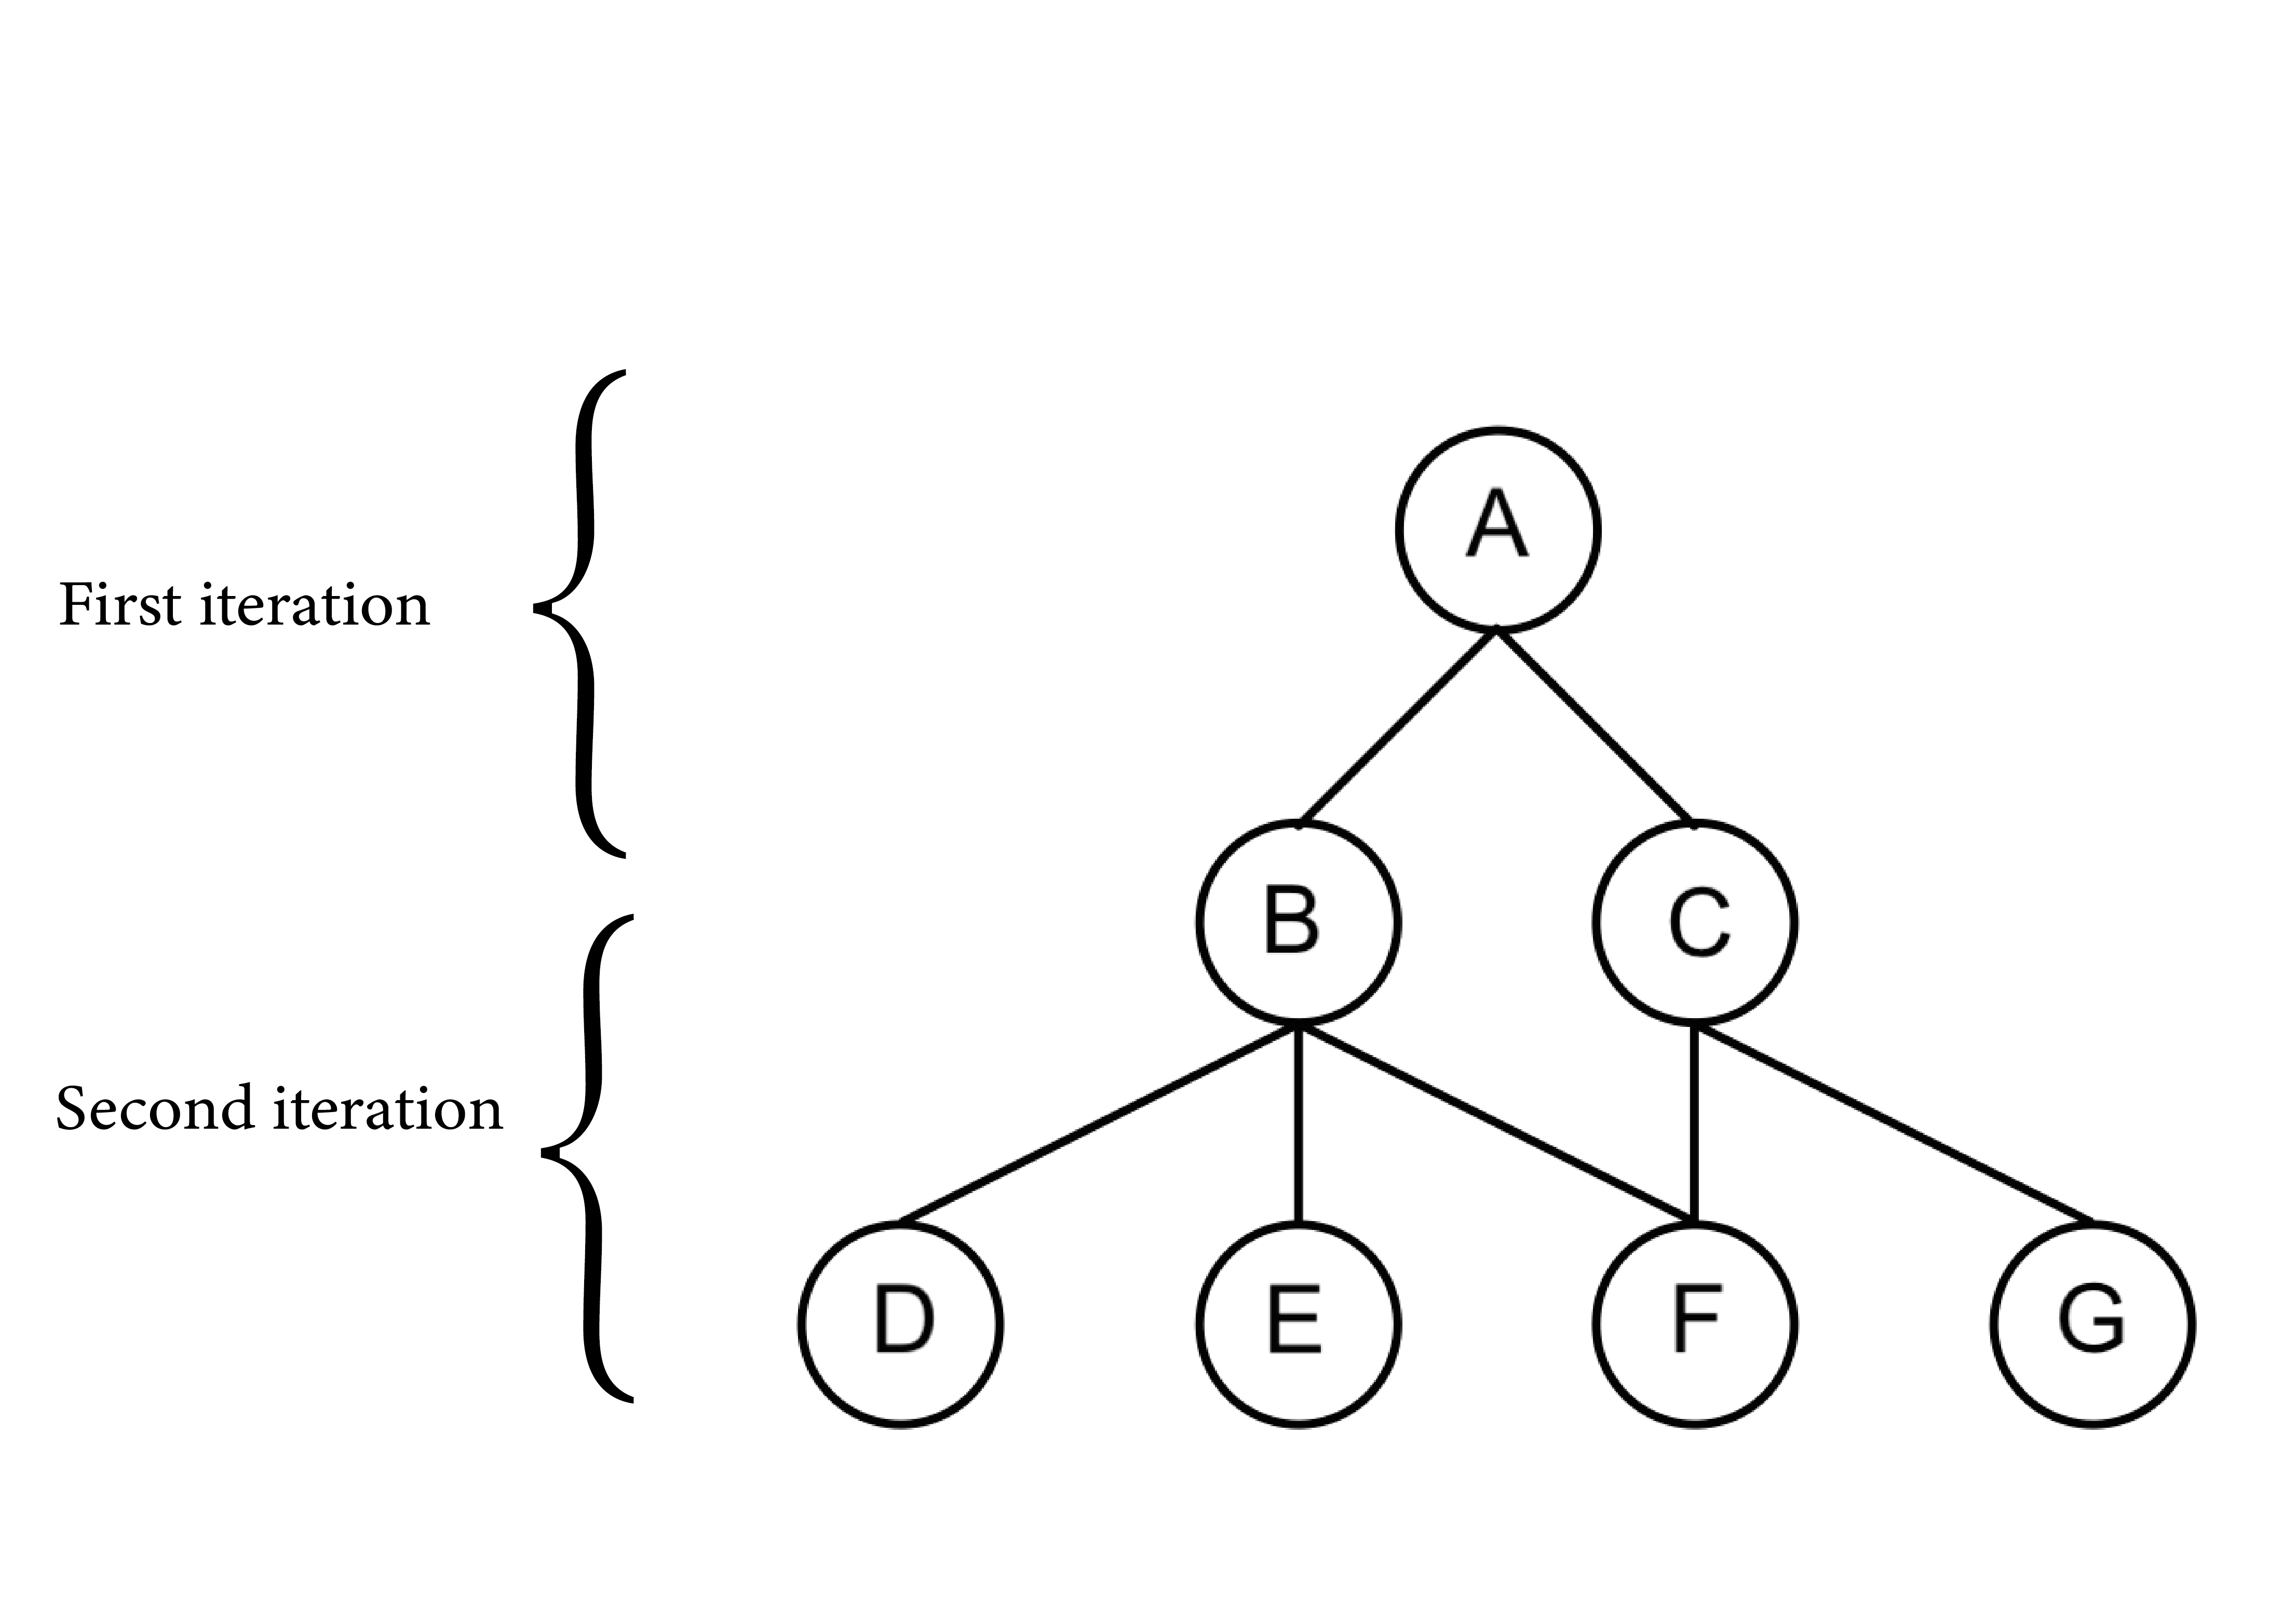
\includegraphics[scale=0.3]{sample_example.png}
	\caption{Snowball process with two iterations}
	\label{fig:snowball}
\end{figure}
\vspace{20pt}

Now let us make some considerations. In our example we started from channel A as seed channel. It is not necessary to start with only one channel; on the contrary. We can take a set of several seed channels. In addition, to make the network more complete we can give a direction to the links. If a message is forwarded from channel A to channel B, the link then will have a direction A$\rightarrow$B. Finally, more than one message can be forwarded between two channels. Channel B may have forwarded hundreds of messages to channel A, while channel C may have forwarded only one message to channel A. This is an important aspect to consider. Therefore, we can add a weight to the link between two channels, which corresponds to the number of messages that was forwarded from one channel to the other.\\

The final result is a network in the form of an edgelist, so a list of links that make up the network. In practice, it is a table with three columns which looks like this:

\renewcommand{\arraystretch}{1.2}

\begin{table}[ht]
\centering
\begin{tabular}{| c | c | c |}
	\hline
	\textbf{source channel} & \textbf{target channel} & \textbf{weight} \\
	\hline
	B & A & 144 \\
	C & A & 81 \\
	E & B & 79 \\
	\hline
\end{tabular}
\caption{Edgelist example}
\label{tab:sample}
\end{table}

\section{Data overview}
We used snowball sampling to study the relationship between online and incel far-right communities. Unlike the example cited above, we started from a set of two seed channels and performed three iterations. For all channels involved we collected messages forwarded over a six-month period – specifically from the 1\textsuperscript{st} of October 2023 to the 2\textsuperscript{nd} of May 2024. We did this three times, using a different pair of seed channels each time. The first time we used two incel channels, the second time two far-right channels, and the last time two far-left channels. The latter serve as a control element, to validate the results obtained\footnote{Due to an unforeseen change in the approach to this work, there is a slight inconsistency in the data collection process. In the case of the Incel network, we did not start from two public channels but from two private groups. Also, the messages for these two groups were not collected from October 1, 2023 but from January 2024. It will be my care to resolve this inconsistency in the future. However, looking at the number of nodes at the end of each iteration, which is similar among the three networks, it is unlikely that this distorted the data.}. The seed channels were chosen arbitrarily. \\

So in the end we get three different edgelists (and thus, three networks): one built from two incel channels, one built from two far-right channels, and one built from two far-left channels. These networks can be thought of as a mapping of information flows from some channels to others. In the next pages, we will refer to these networks as “incel network”, “far-right network”, and “far-left network”. A clarification should be made, however: this does not mean, for example, that all nodes within the incel network actually represent incel channels. In fact, it is likely that they do not. The name “incel network” only indicates that the two seed channels from which the snowball sampling of that network began are two incel channels. The same is true for far-left and far-right. Obviously, we expect that there are more incel channels in the incel network than in the far-right or far-left network – or at least that they have a greater role and exchange activity with the two core channels (which we know for sure are two incel channels). The same reasoning applies to the far-right and far-left networks.\\
The next image shows at each iteration the number of nodes in the networks.
\pagebreak

\begin{figure}[h!]
	\centering
	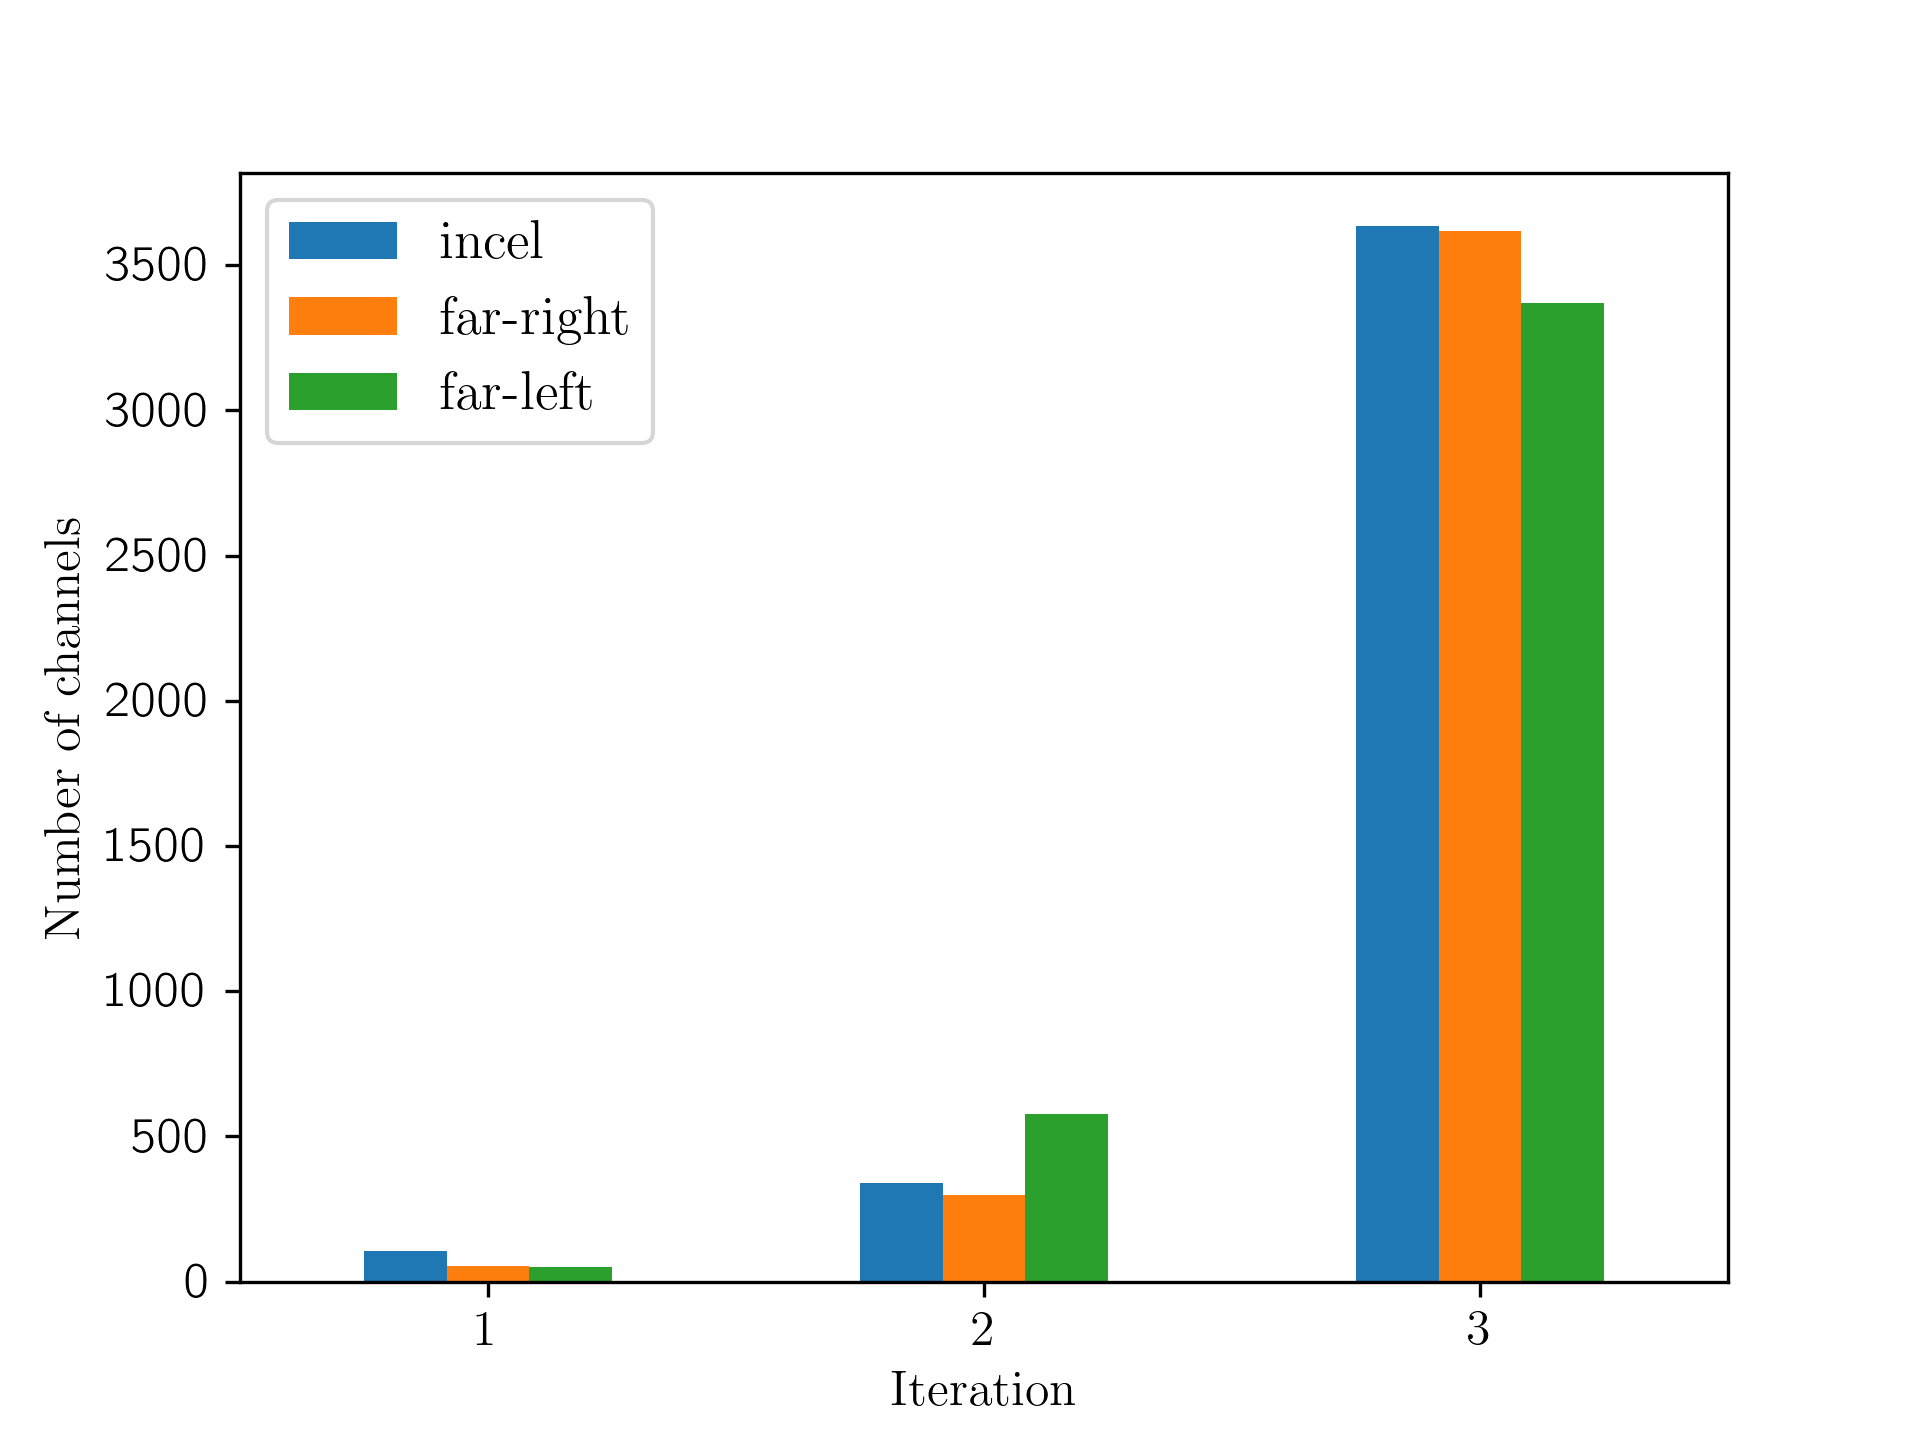
\includegraphics[scale=0.7]{n_nodes_output.png}
	\caption{Number of nodes (i.e.  channels) at each iteration for the different networks}
\end{figure}

After the last iteration, we have 3636 nodes for the incel network, 3616 nodes for the far-left network, 3368 for the far-right network. The mean is 3540. Intuitively, we can see that there are no particular imbalances among the three networks. To make sure of this, we applied a statistical test called “z-score,” which measures how far a certain data point deviates from the mean. It does this by using the standard deviation of the dataset as unit of measurement. In practice, a z-score of \emph{two} for a certain data point would mean that its value deviates by \emph{two} standard deviations from the mean. In general, data points where this indicator is more than 3 or less than -3 are considered outliers. In our case, the results are as follows. In our case, the results are in the table below and confirm that the differences in network sizes are negligible. \\

\renewcommand{\arraystretch}{1.5}
\setlength{\tabcolsep}{2em}
\begin{table}[h!]
	\centering
	\begin{tabular}{| c | c |}
		\hline
		\textbf{network} & \textbf{z-score} \\
		\hline
		incel & 0.64 \\
		\hline
		far-right & 0.50 \\
		\hline
		far-left & -1.15 \\
		\hline
	\end{tabular}
	\caption{Z-scores on the number of nodes in the networks}
\end{table}

\setlength{\tabcolsep}{6pt}

\chapter{Method}
The ultimate goal of this work is to understand whether there is a particular overlap between Incel and far-right communities in Italy. To do so, therefore, we constructed two indicators. The first addresses the overlap between the various networks at the level of individual nodes, while the second considers the structure of the network and the clusters in it.

\section{Node degree overlap}
\label{ch:node_overlap}
Let's start with some basic elements. A network consists of a series of nodes and a series of edges between them. As a result, each node is connected to a number of other nodes.  The number of connections that a certain node has to other nodes in a network is a relevant measure of the its importance and it's called “degree”. So, each node in a network has a certain degree. In the case where links have a direction, the degree of a node can be divided into outdegree and indegree.\\

With all this in mind, the questions we want to answer are: \emph{are there common nodes between the far-right network and the incel network? And what roles do they play in the two networks?}. \\
The underlying assumption is that if there are many nodes in common between the two networks, and that these nodes play an important role in both networks, then information flows in the far-right community and incel community will be similar because they come from the same Telegram channels.\\

Therefore, we found the nodes that are present in the incel network and the far-right network. From these, we eliminated the nodes that are also present in the far-left network, because we are not interested in looking at the nodes that are present in all three. Next, for each of the two networks we see the degree that these common nodes have, compared to the sum of the degree of all nodes in the network. In this way we get an idea of the importance of the common nodes relative to the total. \\
To make the process clearer, we call \(C_{incel}\) the set of all nodes in the incel network. It is defined as \(C_{incel} = \{c_{incel\_1}, c_{incel\_2}, c_{incel\_3},...,c_{incel\_n}\}\). Each of these nodes will have a degree, which is the number of connections it has with other nodes. We call the set of degrees as \(W_{incel}\), which is defined as \(W_{incel} = \{w_{incel\_1}, w_{incel\_2}, w_{incel\_3},...,w_{incel\_n}\}\). Obviously the two sets have the same size, and they are defined so that the degree of node \(c_{incel\_k}\) is \(w_{incel\_k}\). We similarly define the equivalent sets for the other two networks. So we have \(C_{right}\), \(W_{right}\), for the far-right network and  \(C_{left}\), \(W_{left}\) for the far-left network. \\
At this point, we take the nodes that are in \(C_{incel}\) and \(C_{right}\), and that are not in \(C_{left}\) and we call this resulting set \(C_{incel\_right}\). In mathematical notation: 
\begin{displaymath}
	C_{incel\_right} = (C_{incel} \cap C_{right}) - C_{left}
\end{displaymath}


At this point, each element of $C_{incel\_right}$ will correspond to one degree in the incel network and one degree in the far-right network. Mathematically, we can translate this concept with two functions $f$ and $g$ such that 

\begin{align*}
f: C_{incel\_right} \to W_{incel}\\
g: C_{incel\_right} \to W_{right}\\
\end{align*}


Knowing the degree of these nodes gives us an idea of their importance within the two networks. At this point then for both networks we add up the degrees of the common nodes and divide it by the sum of the degrees of all the nodes in the network. Mathematically: 

$$ \frac{
	\sum\limits_{c\in C_{incel\_right}} f(c)
	}
	{
		\sum\limits_{w\in W_{incel}} w
		} $$

and

$$ \frac{
	\sum\limits_{c\in C_{incel\_right}} g(c)
}
{
	\sum\limits_{w\in W_{right}} w
} $$

In the limiting case where the two networks are identical, both values would equal 1. In the case where there are no nodes in common between the two networks, both values would equal 0. \\
We also calculated the same values for the nodes in common between the incel network and the far-left network in order to have a term of comparison. The results are presented in the Results section.

\section{Community separation}
\label{ch:com_sep}

Let us imagine that between two networks there is a significant overlap of nodes, which we have discovered thanks to the indicator just discussed. At this point, however, it could be that these nodes in common are like a small group that has a lot of exchange activity within it, but then they have very little contact with the rest of the network. In this case, the overlapping of nodes would be of much less importance. \\
For this reason, it is useful to combine this first indicator with a measure focusing on network communities. As Radicchi and his colleagues explain with great clarity, \enquote{qualitatively, a community is defined as a subset of nodes within the graph such that connections between the nodes are denser than connections with the rest of the network}\footcite{radicchi2004}. There are many ways to find communities within a network; each method has its strengths and weaknesses. The question behind the measure we are about to define is: \emph{what role do the overlaps between two networks play in their total structure?}.\\
The idea is as follows: let us merge two different edgelists, thus creating a new network. Now, let's see the communities within this network. To which of the two edgelists do they belong, and to what extent? Based on this, we can determine which communities are affected by the overlaps. \\
To get a clearer idea of this, let us look at a limiting case. Assume we create a network in which the only overlaps are very marginal with respect to two groups of densely connected nodes. At this point we find the communities within it. Let us now visualize this network. The result will look like this image below. The color of the nodes indicates the community they belong to, while the color of the connections indicates the edgelist they belong to. 
\pagebreak
\begin{figure}[h!]
	\centering
	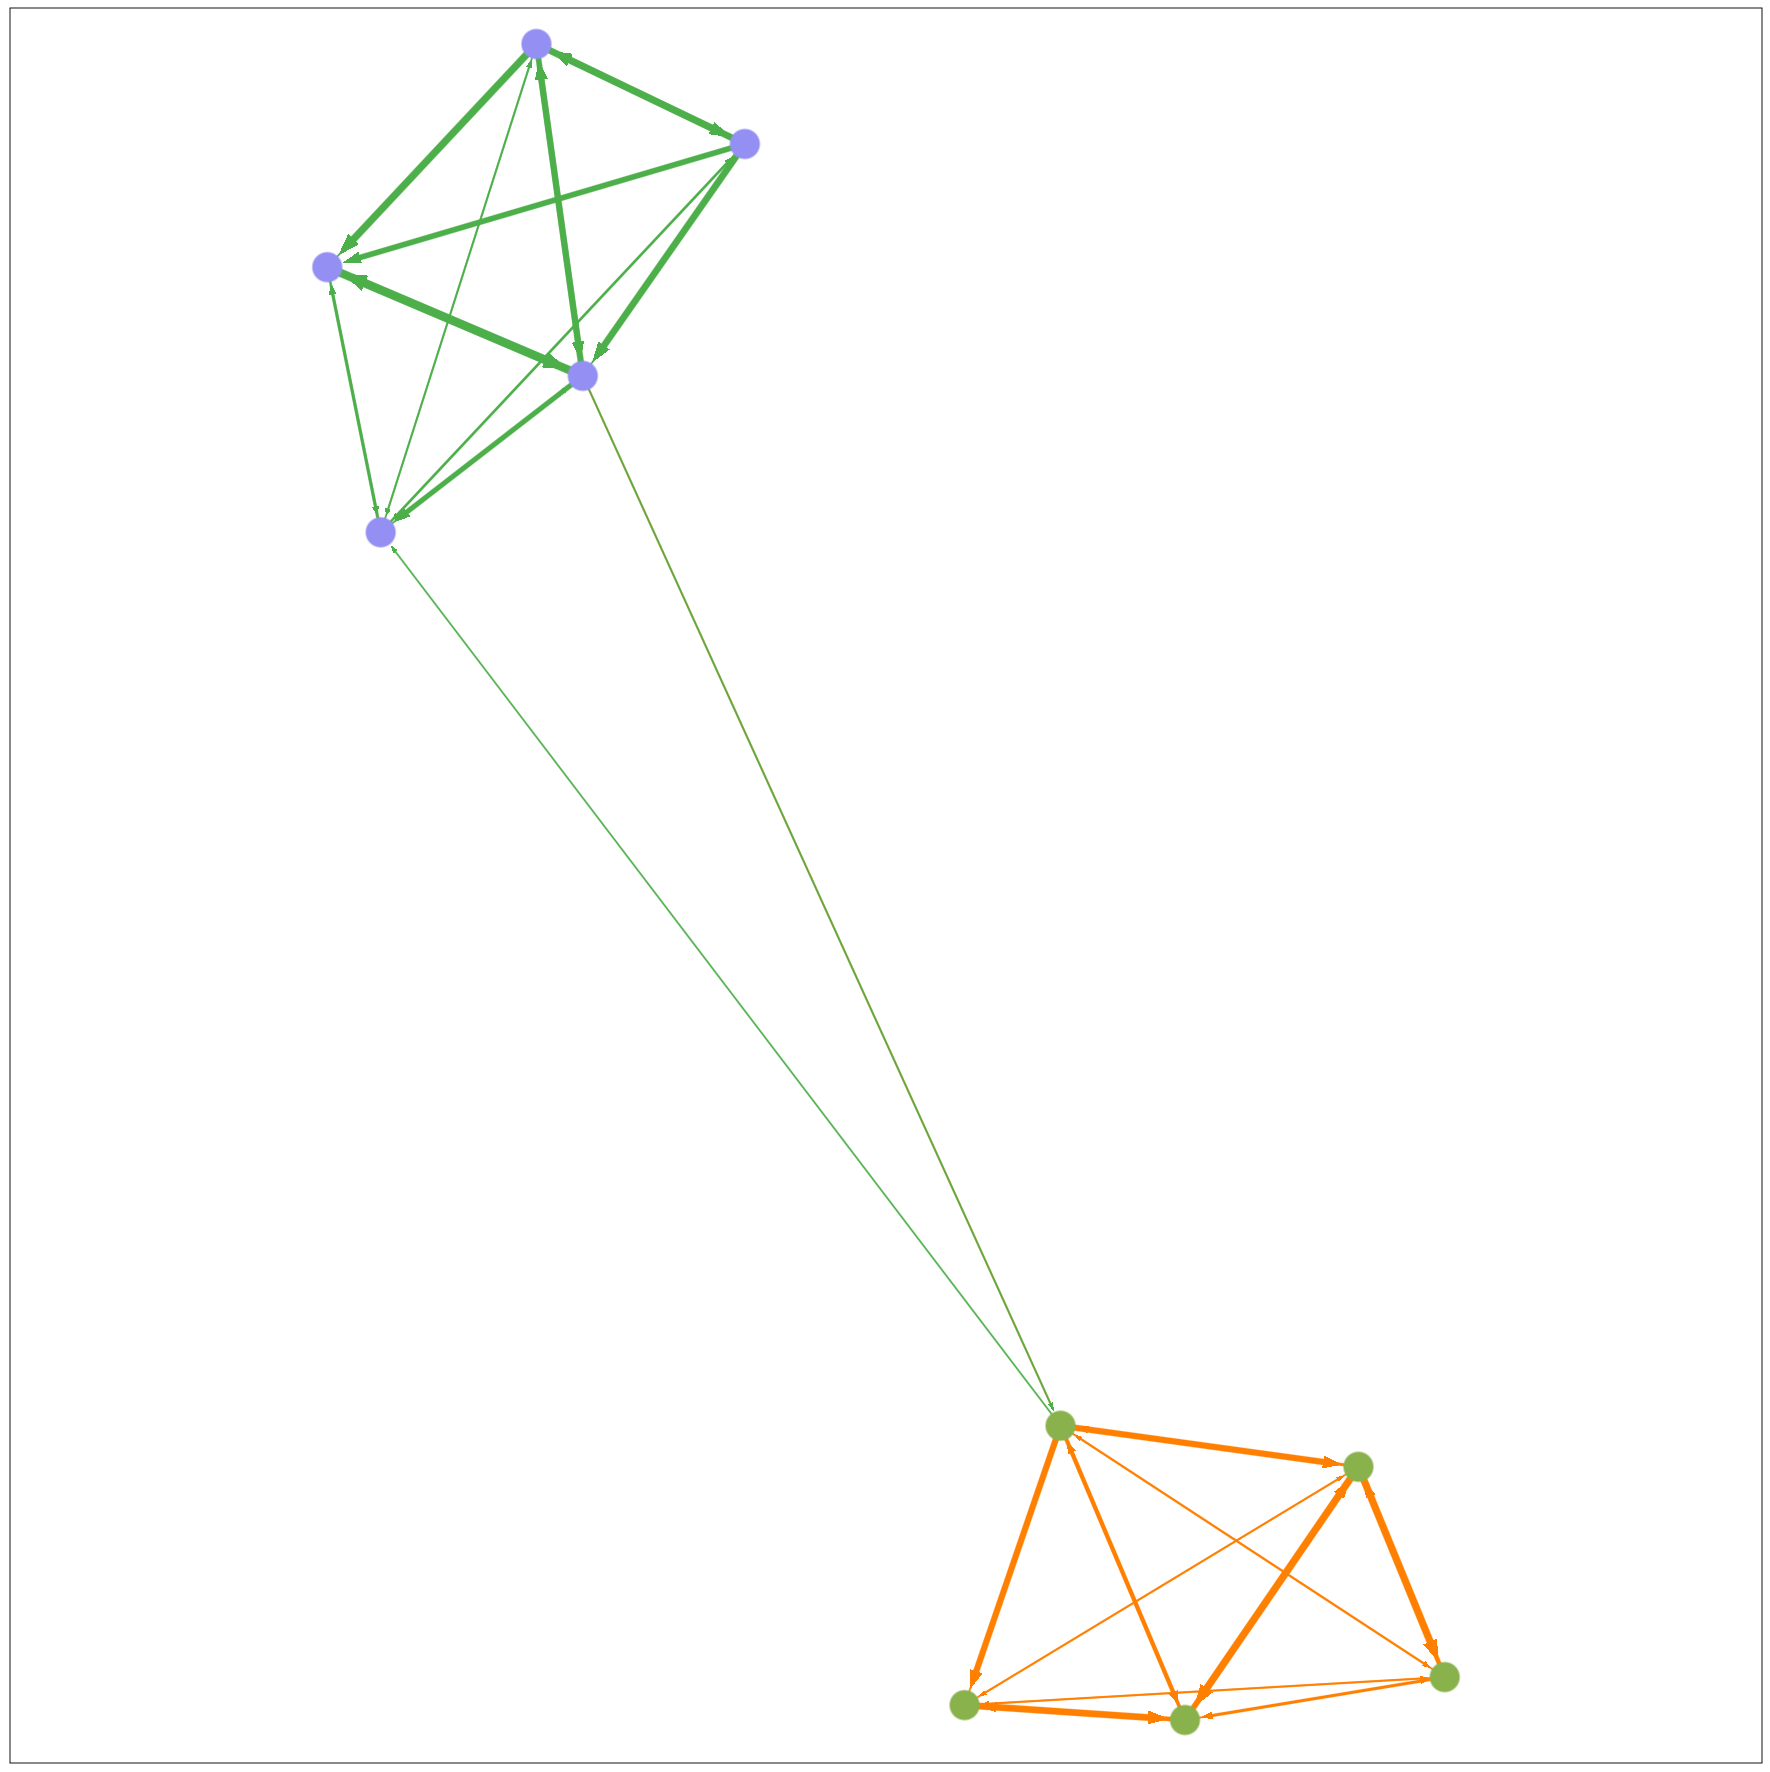
\includegraphics[scale=0.2]{dummy_graph.png}
	\caption{Network created from two almost separate edgelists}
	\label{fig:separate}
\end{figure}

As can be seen, there are two distinct groups of nodes. The two groups also correspond to two different communities, as can be seen by their color. In the two communities, moreover, all connections have the same color. This means that they are all part of the same edgelist. Therefore, it is clear that even if there are overlaps between the edgelists (in other words, some nodes in common), these play a very marginal role.\\
On the other hand, in the case where the two edgelists were not so different, the network would be more like the following image. 
\clearpage

\begin{figure}[h!]
	\centering
	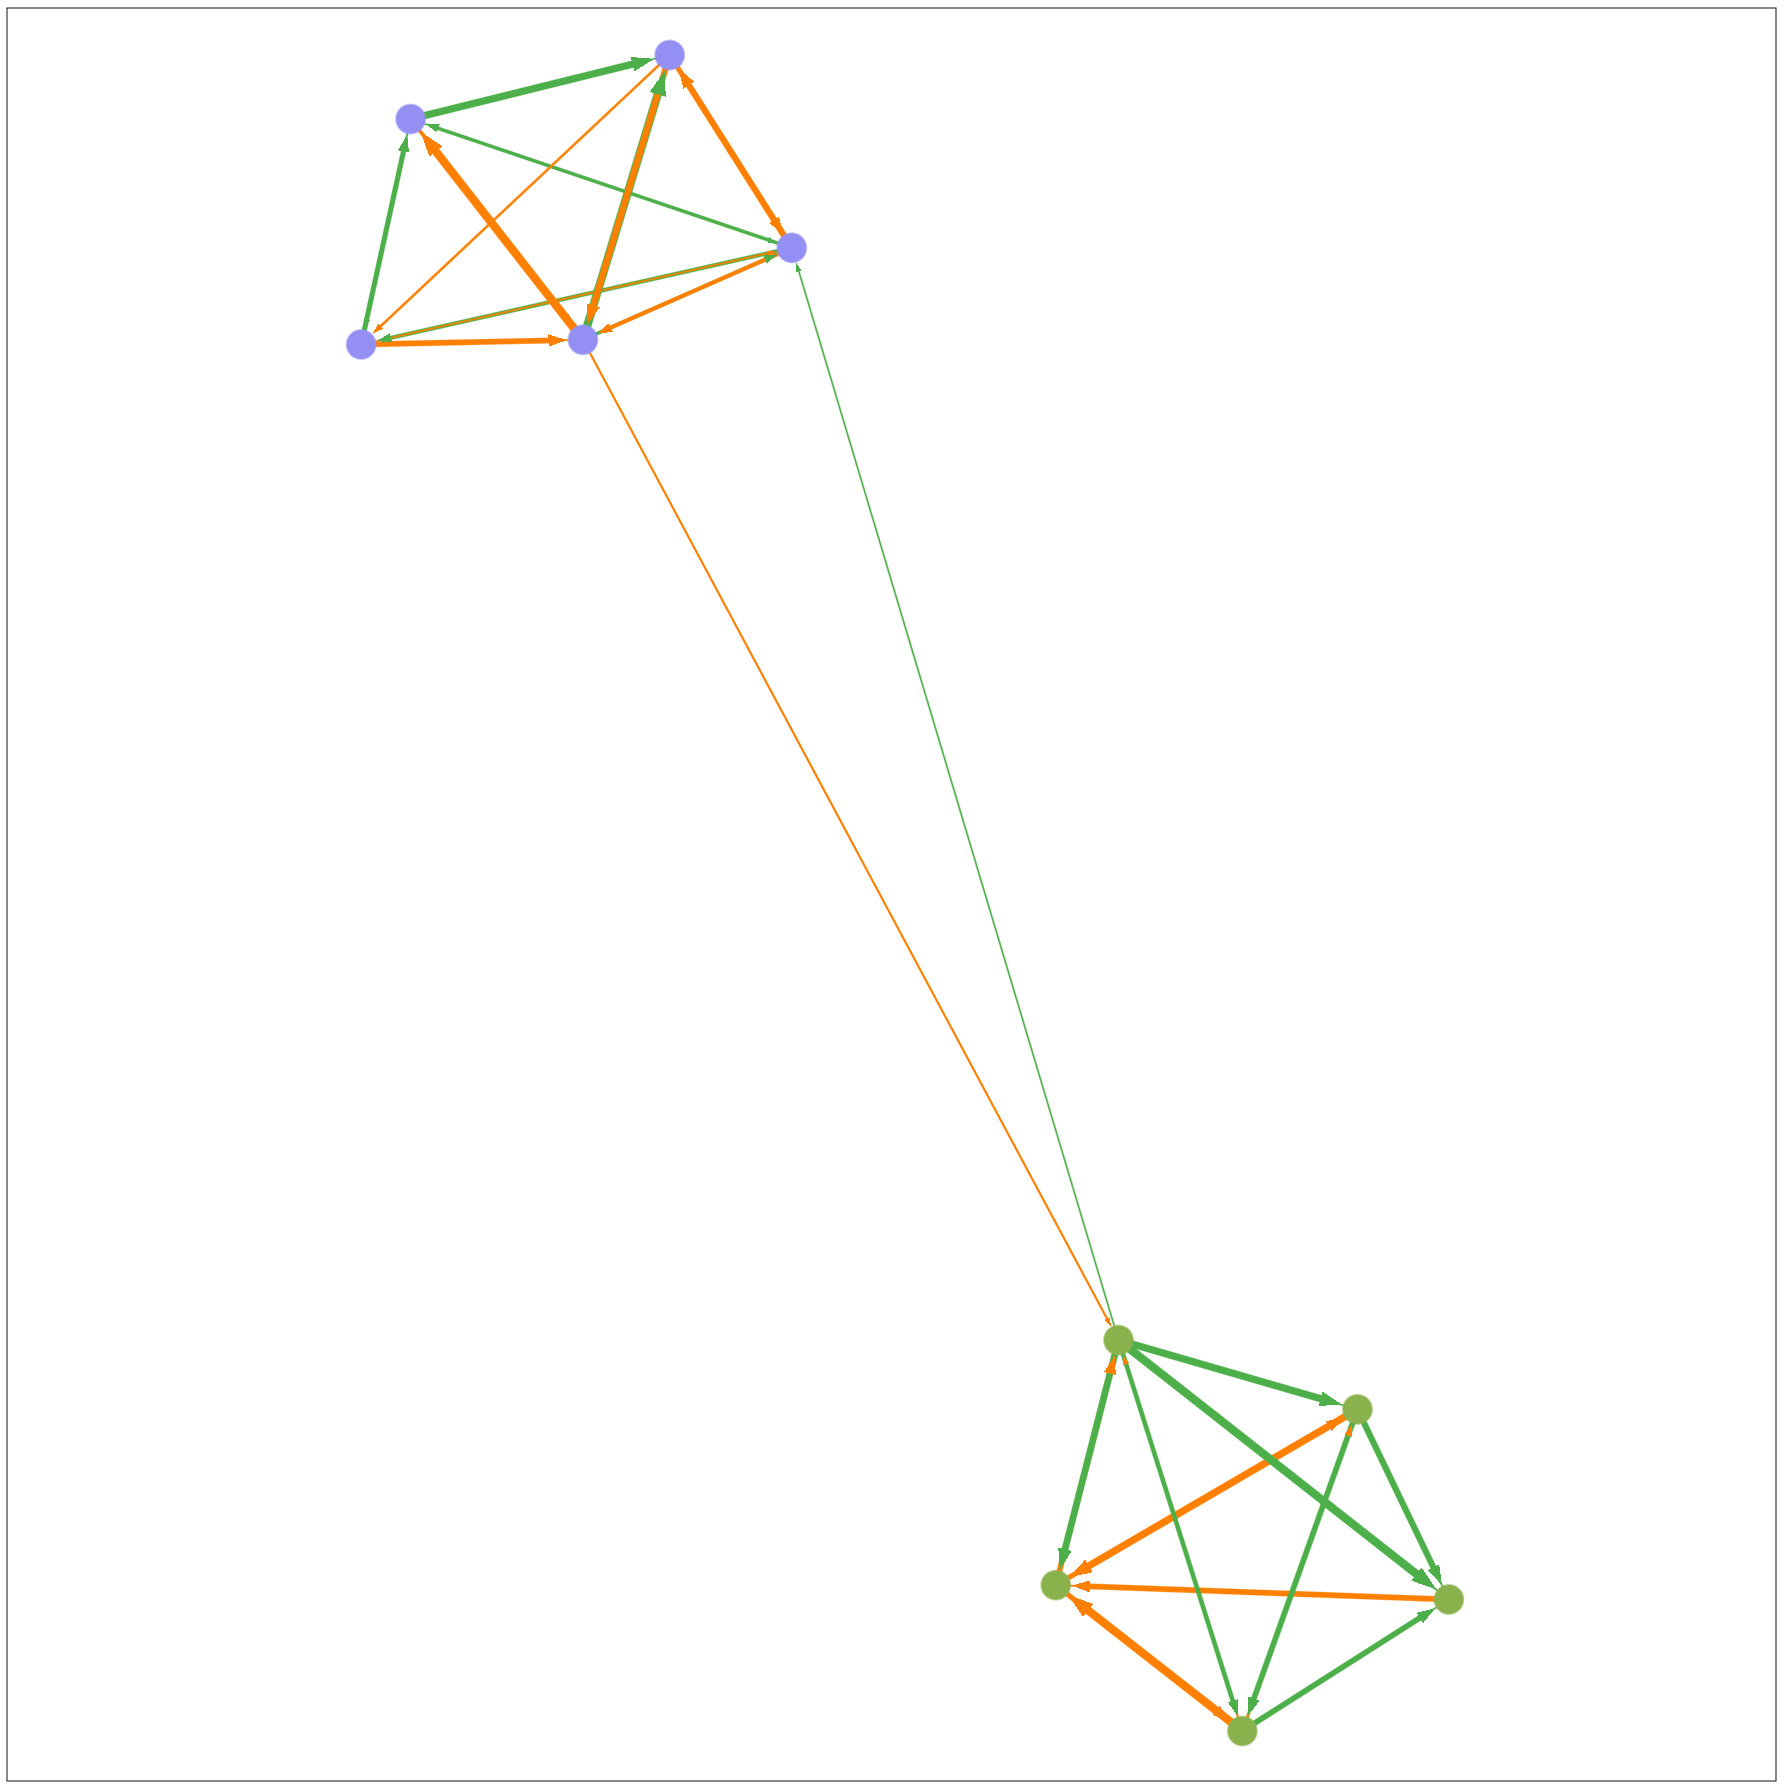
\includegraphics[scale=0.2]{mixed_graph.png}
	\caption{Network created from two edgelists with significant overlaps}
	\label{fig:overlaps}
\end{figure}

Already from the image one can see that the overlaps are much more significant. Within the two communities there are in fact connections of several colours, thus coming from the two different edgelists. The objective of the metric we will define in the following pages is therefore to measure the significance of overlaps between two networks. What we want to do then is to understand what the result is if we combine the incel edgelist with the far-right edgelist and, as an element of comparison, the incel edgelist with the far-left edgelist.\\
In this case, the communities will be a series of telegram channels that have particularly active communication with each other. Seeing whether these communities contain connections largely related to only one of the two edgelists, or whether they are mixed, can give insight into the extent to which the incel and far-right channels have the same information flows.\\

Let us now go into detail. We have three different edgelists: one created from the incel channels, one from the far-right channels, and one from the far-left channels. From these, we can create three different networks. A network consists of two basic elements: a set of nodes C, a set of edges E. In the case of a weighted network, as is our case, another element is added: the function $w: E \to \mathbb{N} $, that simply takes as input an edge and returns the value of its weight. So starting from the three edgelists, we can define: 
\phantomsection
\label{eq:couple_networks}
\begin{align*}
	&G_{incel} = (C_{incel},E_{incel},w_{incel})\\
	&G_{right} = (C_{right},E_{right},w_{right})\\
	&G_{left} = (C_{left},E_{left},w_{left})\\
\end{align*}

Actually, our interest is to combine two edgelists at a time and create the corresponding networks, which means joining the sets nodes and edges. So, for the union of the incel edgelist and the far-right one we have: 

\begin{align*}
	C_{incel\_right} &= C_{incel} \cup C_{right}\\
	E_{incel\_right} &= E_{incel} \cup E_{right}\\
	\text{and then:}\\
	G_{incel\_right} &= (C_{incel\_right}, E_{incel\_right}, w_{incel\_right})\\
\end{align*}
where the function $w_{incel\_right}$ takes as input an edge that belongs to $E_{incel}$ or $E_{right}$ and returns its correspondent weight in the network it belongs to, thus $G_{incel}$ or $G_{right}$. Formally it is defined as follows:
\begin{align*}
	w_{incel\_right}(x) = 
	\begin{cases} 
		w_{incel}(x) & \text{if } x \in E_{incel} \\
		w_{right}(x) & \text{if } x \in E_{right}\\
	\end{cases}
\end{align*}

And similarly we can define the equivalent of the union between the incel edgelist and the far-left one $G_{incel\_left} = (C_{incel\_left}, E_{incel\_left},w_{incel\_left})$. For the sake of explanation, however, let us momentarily consider only the case of network $G_{incel\_right}$. We use a random walk algorithm to find communities within this network\footnote{The choice of the algorithm to be used was conditioned by the literature on the subject. A more robust selection criterion should be found to validate the results. This will be explored more in the section on the limits in this work.}. This results in $n$ communities. Each community is defined as a smaller network within the initial network. In the case of $G_{incel\_right}$, for each $i$ from 0 to $n$, the $i$-th community can be formally written as: 

\begin{align*}
	&H_{i}= (C_{com\_i}, E_{com\_i}, w_{incel\_right})\\
	\text{where:}\\
	&C_{com\_i} \subseteq C_{incel\_right}\\
	&E_{com\_i} \subseteq E_{incel\_right}\\
\end{align*}

At this point, what we are interested in is how many edges of the $i$-th community are contained in the incel edgelist and how many in the far-right edgelist. In essence, then, it is a matter of finding the intersections between the sets of edges among the various networks. Which means:

\begin{align*}
	&E_{com\_incel\_i} = E_{com\_i} \cap E_{incel}\\
	&E_{com\_right\_i} = E_{com\_i} \cap E_{right}\\
\end{align*}

We now want to discover the importance that the two sets we just found have with respect to the total number of edges within the community. To do this, we use the weights of the edges through the $w_{incel\_right}$ function. We are interested in looking at the relationship between the two numbers, whether they are closer to a condition of equality or whether there is a large imbalance instead. What can be called as the \enquote{degree of separation} of the $i$-th community will then be the largest number in the pair. 
So, formally:

\begin{align*}
	\max
	\left(
	\frac{
		\sum\limits_{
	x \in E_{com\_incel\_i}
	} w_{incel\_right}(x)}
{
	\sum\limits_{
		x \in E_{com\_i}
	} w_{incel\_right}(x)} \, \mathpunct{;} \,
\frac{
	\sum\limits_{
		x \in E_{com\_right\_i}
	} w_{incel\_right}(x)}
{
	\sum\limits_{
		x \in E_{com\_i}
	} w_{incel\_right}(x)}
\right)
\end{align*}
\\
The values this number can take range from 0.5 (the case of “perfect” mixing) to 1 (the case of maximum separation). To make it easier to understand, we applied a normalization to fit a 0 to 1 scale. So, after normalization, the value of "perfect mixing" is 0 and the case of maximum separation is 1. Consequently, the average value of this index for the two communities in the network in figure \ref{fig:separate} is equal to 1, while the same index for the network in \ref{fig:overlaps} has an average of 0.06 for the two communities.
\\
In the Results section, we will calculate these values for the 10 largest communities in the $G_{incel\_right}$ network and the equivalents for the $G_{incel\_left}$ network, so that comparisons can be made. 

\chapter{Results and discussion}
\section{Node degree overlap}
\label{sec:node_degree}
We calculated the degree overlap for nodes in common between the incel network and the far-right network. This means that we have two values: the weight that these nodes have on the total incel network and the weight that these nodes have on the total far-right network. Numbers are presented as percentages.
\\

\renewcommand{\arraystretch}{1.5}

\begin{table}[h!]
\centering
	\begin{tabular}{| c | c |}
		\hline 
		Incel network & Far-right network \\ 
		\hline 
		19.4\% & 18.4\% \\ 
		\hline
	\end{tabular}
	\caption{Node degree overlap between incel and far-right networks}
\end{table}

As can be seen, the two numbers are quite similar. Nodes in common between the two networks account for approximately 18-19\% of the total in both networks. Now let's do the same for the nodes in common between the incel and far-left networks.
\\

\begin{table}[h!]
	\centering
	\begin{tabular}{| c | c |}
		\hline 
		Incel network & Far-left network \\ 
		\hline 
		11.2\% & 6.0\% \\ 
		\hline
	\end{tabular}
	\caption{Node degree overlap between incel and far-left networks}
\end{table}

Comparing the two tables, it can be seen that the nodes shared by the incel and far-left networks cover a much smaller portion of the total than the nodes shared by the incel and far-left networks. This shows that there is a greater closeness between the flow of information around Telegram incel channels and far-right ones than those of the far-left. \\
That is not all. In the case of nodes in common between incel and far-left networks, there is also an internal difference to consider. The nodes that in the incel network cover 11.2\% of the total, in the far-left network cover only 6\%, almost half. This means that these common nodes are even less important within the far-left information flows.

\section{Community separation}
\label{ch:com_results}
We calculated the \enquote{degree of separation} of the 10 largest communities in networks $G_{incel\_right}$ and $G_{incel\_left}$\footnote{These networks were defined in the Method section, precisely at page \pageref{eq:couple_networks}}. We then calculated the weighted average of the 10 values for the two networks, using the number of nodes in each community as weights. The results, in percentages, are as follows:
\\

\begin{table}[h!]
	\centering
	\begin{tabular}{| c | c |}
		\hline 
		$G_{incel\_right}$ & $G_{incel\_left}$ \\ 
		\hline 
		80.1\% & 94.7\% \\ 
		\hline
	\end{tabular}
	\caption{Weighted average of degree of separation for the 10 largest communities in the two networks}
\end{table}

The results are consistent with the values in \ref{sec:node_degree}. In fact, the degree of separation for the 10 largest communities in the $G_{incel\_right}$ network is lower than for the $G_{incel\_left}$ network. This means that the information flows in the most active communities associated with incel channels are more similar to those of far-right channels than to those of far-left ones. To add more robustness to these results, we checked the value of the average degree of separation if more or fewer communities are considered. The following graph shows the average degree of separation of the first $n$ largest communities in the two networks, with $n$ ranging from 1 to 100. The average values are always weighted on the number of nodes present in each community.

\begin{figure}[h!]
	\centering
	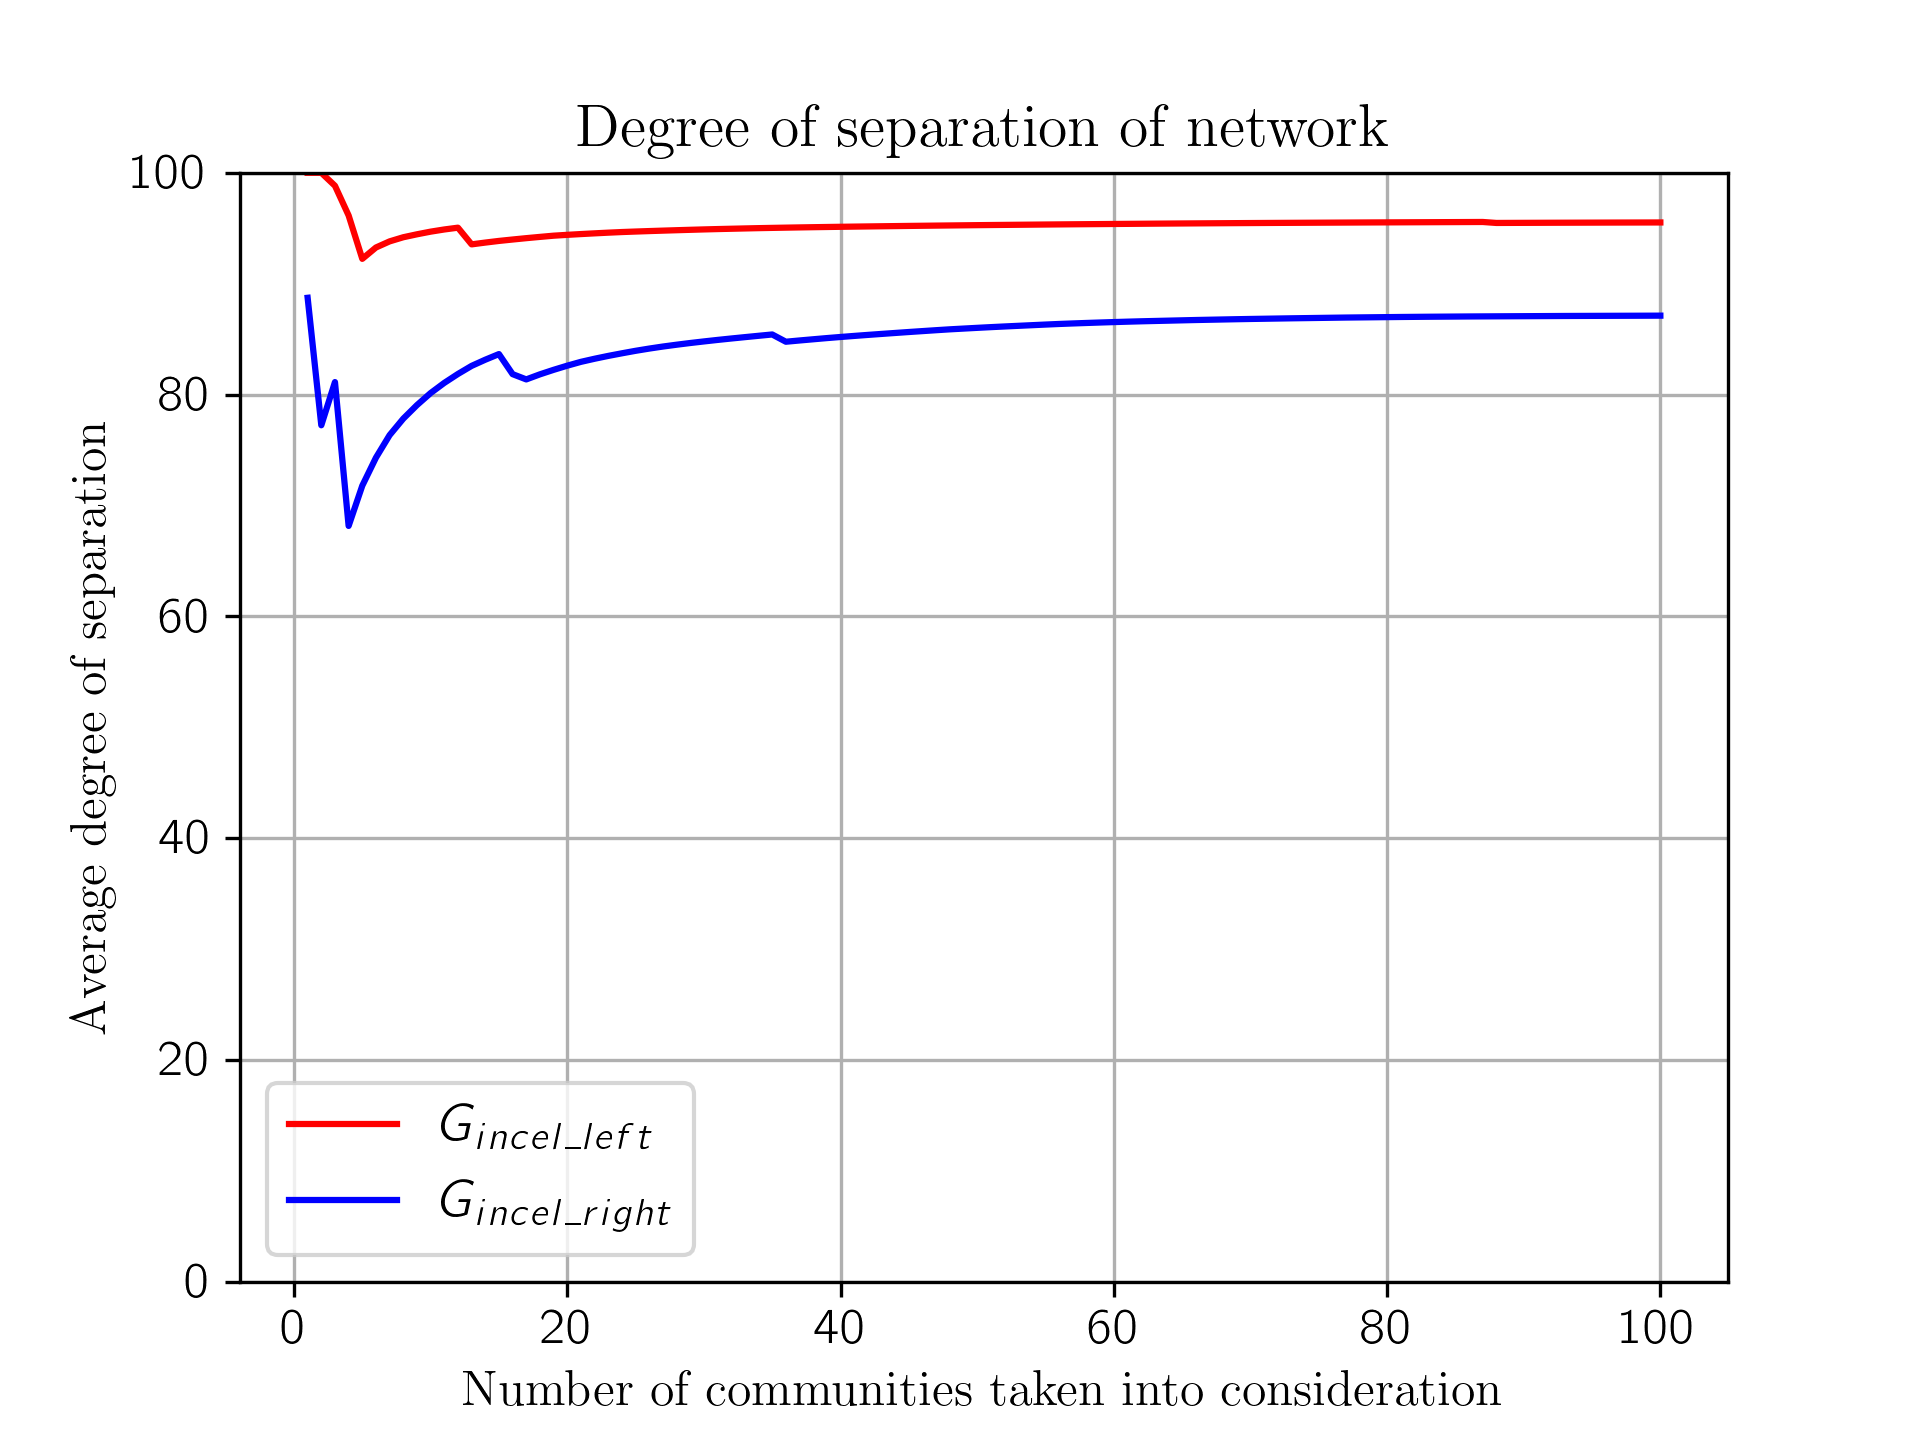
\includegraphics[scale=0.75]{average_degree.png}
	\caption{Average degree of separation of the first $n$ largest communities}
\end{figure}
\pagebreak

As can be seen, the degree of community separation in the $G_{incel\_left}$ network remains higher regardless of the number of communities considered. The maximum gap between the two networks values corresponds to when the first four largest communities are taken into account. Thereafter, the gap tends to decrease as more communities are considered.

\section{Discussion}
Both results confirm the presence of a greater overlap between the network built from Italian incel channels and the one built from far-right channels, compared to the one created from far-left channels. This suggests the presence of an increased exchange of messages and information on Telegram between incel and far-right channels. These results thus confirm previous research on the subject, showing the validity of their findings on the Italian case as well. 

\section{Limits}
There are several limitations of the present work to point out.\\
\textbf{Data collection:} as also pointed out in \ref{ch:data}, the data collection method used in this work has a slight inconsistency, due to an unforeseen change in the approach to this work. In the case of the Incel network, we did not start from two public channels but from two private groups. Also, the messages for these two groups were not collected from October 1, 2023 but from January 2024.\\
\textbf{Networks creation:} the results obtained are highly dependent on the data collected and the way in which the snowball sampling iterations were conducted. More in-depth work should validate the results using the same snowball sampling methodology starting from several different channel cores of different sizes.\\
\textbf{Community detection:} communities used in \ref{ch:com_sep} were identified through a random walk algorithm. The results in \ref{ch:com_results} are highly dependent on the way communities within the networks are identified. More work should be done to select the most suitable methodology and to ensure that the results are also consistent using other algorithms.\\
\textbf{Metrics interpretability:} while the indicator established in \ref{ch:node_overlap} is quite simple in its definition, the measures created in \ref{ch:com_sep} are overly elaborate. Further research is needed to define more appropriate methodologies for analyzing the structure of telegram channel interactions.

\chapter{Code}
All the code used is available here: \url{https://github.com/savaij/M1\_memoire}


\backmatter


\titleformat{\chapter}[display]
{\normalfont\bfseries}{}{-3em}{\Huge}

\listoffigures
\listoftables
\tableofcontents

\end{document}
